\chapter{Survey}
\label{chapter:survey}

This chapter will discuss the creation of the questionnaire, showing its pretest and the final version, and then discuss the results obtained.

As mentioned on Section \ref{sec:goodmap} of Chapter \ref{chapter:proposal}, a survey was developed in order to test if a number of our generated maps can achieve the criteria we defined for what makes a good generated map; while also making the use of the ARCS model, which is used to evaluate the participants' motivation to play a game using the generated maps. 

Both questionnaires were made available through Google Forms in Brazilian Portuguese. They make use of the typical five-level Likert scale:
\begin{itemize}
    \item Strongly disagree.
    \item Disagree.
    \item Neither agree nor disagree.
    \item Agree
    \item Strongly agree.
\end{itemize}

Both questionnaires start with a question about the participant age group, and a question about how familiar they are with 2D top-down games. Also in both, participants were asked to carefully visualize eight different maps generated by our system, these images are available in Appendix \ref{appendix:a}. The main concern during the generation of these maps was to create varied results by tweaking the user-defined parameters of the system.

Translated versions of the questionnaires are made available in Appendix \ref{appendix:b} and Appendix \ref{appendix:c}. The justification of each question is also presented. Details about both of them will be discussed in the next sections, as well as their results.
 
\section{Pretest questionnaire}

Before sharing a definitive version of the questionnaire, a pretest was made with a smaller group of participants.

The pretest had 23 participants. These were the first two questions, made with the purpose of understanding the profile of the respondents:
\begin{itemize}
    \item What is your age group (in years)?
    \begin{itemize}
        \item \emph{(18-)} Less than 18.
        \item \emph{(18 - 25)} Between 18 and 25.
        \item \emph{(26 - 30)} Between 26 and 30.
        \item \emph{(31 - 35)} Between 31 and 35.
        \item \emph{(35+)} More than 35.
    \end{itemize}
    \item How familiar are you with 2D top-down games? (games like Zelda, Pokémon, Bindings of Isaac, Hotline Miami etc)
    \begin{itemize}
        \item \emph{(1)} Never heard of it.
        \item \emph{(2)} Heard of it, but never played.
        \item \emph{(3)} I've seen videos of people playing this type of games.
        \item \emph{(4)} I've played at least one game in this style.
        \item \emph{(5)} I've played more than one game in this style.
    \end{itemize}
\end{itemize}

\begin{figure}[h]
  \centering
  \begin{minipage}[b]{0.4\textwidth}
    \caption{Age group of participants.}
    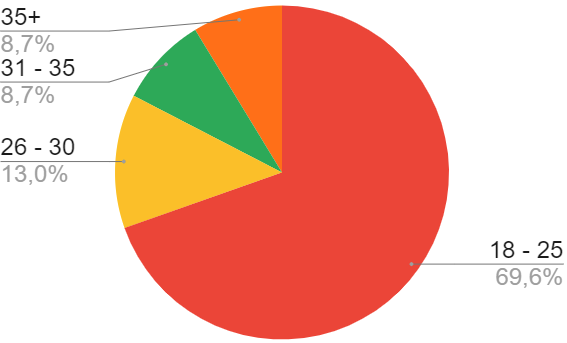
\includegraphics[width=\textwidth]{images/survey/pretest_age.png}
    \legend{Source: Image provided by author}
    \label{fig:pre_age}
  \end{minipage}
  \hfill
  \begin{minipage}[b]{0.4\textwidth}
    \caption{Participants' familiarity with 2D top-down games.}
    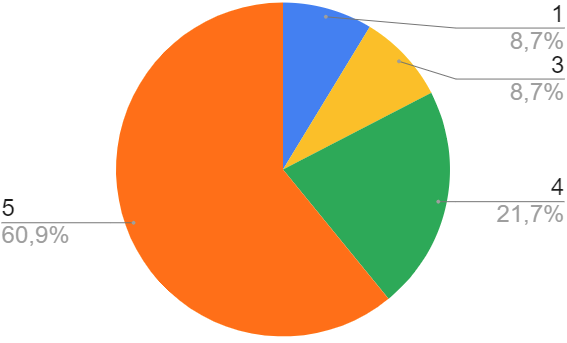
\includegraphics[width=\textwidth]{images/survey/pretest_played.png}
    \legend{Source: Image provided by author}
    \label{fig:pre_game}
  \end{minipage}
\end{figure}

The results of these questions are shown here in Figure \ref{fig:pre_age} and Figure \ref{fig:pre_game}. We had the participation of mostly young people who were already familiar with the concept. This is important since, according to \cite{statista:2017}, a 2017 survey showed that the majority of gamers are from the age group of 21 - 35 years.

After these initial questions, as mentioned before, participants were asked to carefully visualize the map images shown in Appendix \ref{appendix:a}, then responded the 15 questions regarding the map, available in Appendix \ref{appendix:b}. Also in Appendix \ref{appendix:b} is the next part of the pretest, which involves answering five subjective questions about the questionnaire itself, shown in Table \ref{table:pretest_quest}.

\subsection{Pretest results}

For the pretest, the results we analyzed are the ones about the questionnaire itself, i.e., the ones in Table \ref{table:pretest_quest}. All of the points listed here have been taken into account when developing the second version.

\subsubsection{Question 1}

Question 1 reads: "Do you think that the questions from this questionnaire were easy to understand? If not, why?".

This question had 12 answers, from which 7 were positive, 3 were negative and 2 were neutral. The most important points we gathered from the neutral and negative answers were:

\begin{itemize}
    \item Participants weren't sure what the map would be used for, this made it harder for them to answer the questions.
    \item Participants who were unfamiliar with 2D top-down games found it hard to visualize how the maps could be explored.
\end{itemize}

\subsubsection{Question 2}

Question 2 reads: "Are there repeated questions in this questionnaire? If yes, which?".

This question had 17 answers, from which 9 were negative and 8 were positive. All of the positive answers referred to questions that were opposites from one another, for example, question 9 (The generated map’s design made it difficult for me to keep my attention.) and 10 (The generated cave maps were capable of capturing my attention.).

\subsubsection{Question 3}

Question 3 reads: "Would you include other questions on this questionnaire? If yes, which?".

This question had 16 answers, from which 7 were negative and 9 were positive. Most of these 9 positive answers suggested some type of comparison between the maps. From our understanding, adding questions that compare the generated maps is beyond the scope of this work, therefore we concluded that we need to better explain the objectives of the work before asking the questions.

One of the suggestions was to add a demonstration of how a character would view these maps, how far away would the camera be, how much of the map could be seen etc. 

\subsubsection{Question 4}

Question 4 reads: "Would you change the text of one or more questions in this questionnaire? If yes, which?".

This question had 14 answers, from which 7 were negative and 7 were positive. The most important points gathered from the positive answers are listed here:
\begin{itemize}
    \item Grammatical errors to be corrected.
    \item Use a more direct language.
    \item Change questions 7 and 8 so that, instead of being either one or the other, we can measure the influence of each separately.
\end{itemize}

\subsubsection{Question 5}

Question 5 reads: "Do you think a question comparing the generated maps to real cave representation is necessary for this questionnaire?".

This question had 19 answers, from which 13 were positive and 6 were negative. Some of the positive answers suggested showing some real cave patterns, arguing that it can be difficult to imagine how the structure of a cave can be represented in 2D.

\section{Second version of questionnaire}

After reviewing all the suggestions and important points brought up on the pretest questionnaire, we developed a second improved version, which can be seen on Table \ref{table:final_quest} of Appendix \ref{appendix:c}.

The second version had 163 participants, the first two questions were the same as the ones asked in the pretest, their results can be seen in Figure \ref{fig:age} and in Figure \ref{fig:gamekn}. We can see by these results that the participants' profile is the same from the pretest.

\begin{figure}[h]
  \centering
  \begin{minipage}[b]{0.4\textwidth}
    \caption{Age group of participants.}
    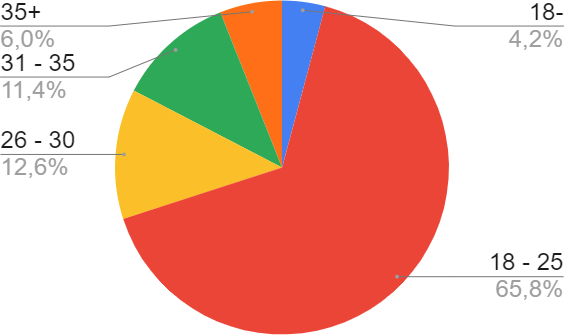
\includegraphics[width=\textwidth]{images/survey/age.png}
    \legend{Source: Image provided by author}
    \label{fig:age}
  \end{minipage}
  \hfill
  \begin{minipage}[b]{0.4\textwidth}
    \caption{Participants' familiarity with 2D top-down games.}
    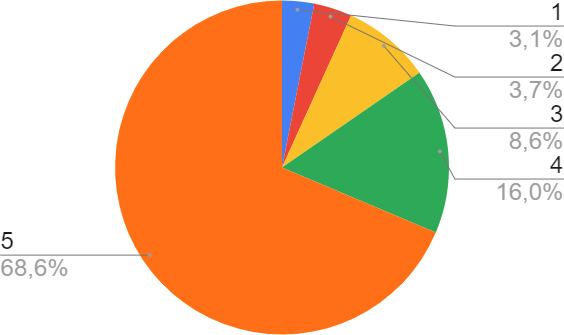
\includegraphics[width=\textwidth]{images/survey/played.png}
    \legend{Source: Image provided by author}
    \label{fig:gamekn}
  \end{minipage}
\end{figure}

A new question was added with the intent of identifying the profile of the participants: "Did you ever participate in the development of a video game?". For which 41,1\% answered positively and 58,9\% answered negatively. This is relevant since, as discussed on Section \ref{sec:pcg} of Chapter \ref{chapter:intro}, one of the main objectives of PCG in video games is to assist in game design.

After these three initial questions, the participants were given a summary of the objectives of this work, along with the image from Figure \ref{fig:cave_patterns}, to assist in answering the questions to come. Additionally, an animated GIF of a character walking around one of the generated maps was added, a still image of this GIF can be seen here on Figure \ref{fig:gif}.

\begin{figure}[h]
    \caption{Still frame of GIF shown to participants, showing a character walking on a generated map.}
    \centerline{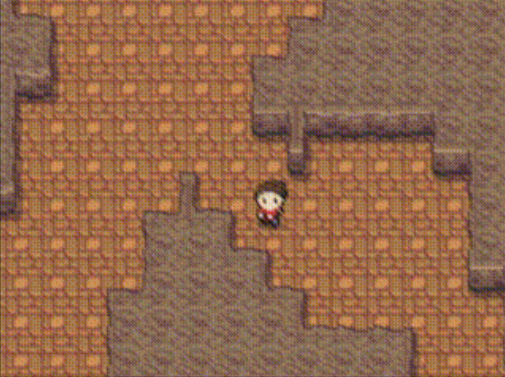
\includegraphics[width=8cm]{images/survey/gif.png}}
    \legend{Source: Image provided by author}
    \label{fig:gif}
\end{figure}

\subsection{Results}

To analyze the results, we assigned a weight to each option of the Likert scale, from 1 (strongly disagree) to to 5 (strongly agree). The question's proposition was considered satisfied if the average of answers achieved 60\% of the ideal value. For some questions the ideal is to reach 5, for others the ideal is to reach 1. Therefore, considering \(MAX\) as the maximum answer, \(MIN\) as the minimum answer, and \(V_{max}\) and \(V_{min}\) as the maximum and minimum satisfactory value, respectively:

\begin{center}
\(V_{max} = (MAX - MIN) * 0.6 + MIN = (5 - 1) * 0.6 + 1= 3.4\)
\(V_{min} = (MAX - MIN) * 0.4 + MIN = (5 - 1) * 0.4 + 1 = 2.6\)
\end{center}

The average and mode of the answers is shown on Figure \ref{fig:final_res}, where the questions that have the ideal value as 5 are marked with a \emph{(+)} after the question number, and the ones that have the ideal value as 1 are marked with a \emph{(-)}.

\begin{figure}[h]
    \caption{Average and mode of the second version questionnaire.}
    \centerline{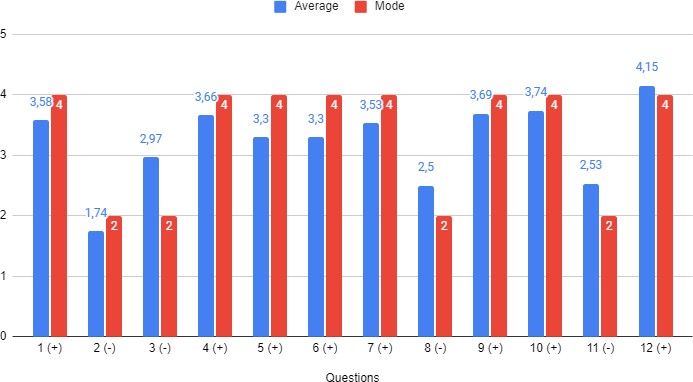
\includegraphics{images/survey/final_results.png}}
    \legend{Source: Image provided by author}
    \label{fig:final_res}
\end{figure}

By these metrics; questions 1, 2, 4, 7, 8, 9, 10, 11 and 12 have reached a satisfactory result; while questions 3, 5 and 6 have not.

Out of the questions that have reached satisfactory results, the most important points gathered were:
\begin{itemize}
    \item All of the questions related to the ARCS model for measuring motivation have reached satisfactory results.
    \begin{itemize}
        \item Attention was shown to be the least influential component (questions 1 and 8).
        \item Confidence and relevance were the major drivers for motivation (questions 2 and 12).
    \end{itemize}
    \item The structure of the caves was shown to be slightly more important in achieving the natural look for the map (question 7).
    \item The variety criteria didn't reach a very expressive result, although still below the 40\% mark. (question 11).
    \item The criteria that proposed that the generated maps should encourage players to explore was reached by a good margin (question 9).
\end{itemize}

Out of the questions that haven't reached satisfactory results, the most important points gathered were:
\begin{itemize}
    \item It would be easy to get lost on the generated maps (question 3).
    \begin{itemize}
        \item This could be attributed to the labyrinthic nature of caves.
        \item Generating larger maps tend to create many branching paths. This can mean that the system is more effective when generating smaller maps.
    \end{itemize}
    \item Even though the results of question 4 suggests that the system can generate natural-looking structures, the result of question 5 suggests that the maps still don't quite look like real caves. Although the result was not drastically low. 
\end{itemize}